\subsection{Adaptaci�n}
\begin{frame}

\frametitle{}

\begin{figure}
\begin{tikzpicture}[node distance=0.5cm, auto,>=latex', thick]
\scriptsize
    % We need to set at bounding box first. Otherwise the diagram
    % will change position for each frame.
    \path[use as bounding box] (-1.5,0) rectangle (12,-2);

    % TT methodology     
    \node [phase]                        (monitoreo)     {Vigilancia};
    \node [phase, below of=monitoreo]    (choice)        {Elecci�n};
    \node [phase, below of=choice]       (acquisition)   {Adquisici�n};
    \node [phase2,below of=acquisition]  (adaptation)    {Adaptaci�n};
    \node [phase, below of=adaptation]   (absortion)     {Absorci�n};
    \node [phase, below of=absortion]    (aplication)    {Aplicaci�n};
    \node [phase, below of=aplication]   (difusion)      {Difusi�n};

    %%%%%%%%%%%%%%%%%%%%%%%%%%%%%%%%%%%%%%%%%%%%&
    %            Adaptaci�n
    %%%%%%%%%%%%%%%%%%%%%%%%%%%%%%%%%%%%%%%%%%%%&
    \onslide<1> \node [ph_explain, right=.5cm of adaptation.east] (exp_adaptation)    
    {
    \begin{center} \textbf{Adaptaci�n} \end{center}
    \begin{itemize}
     \item Se presenta cuando la sociedad encuentra posible y deseable realizar cambios para involucrar usos particulares de la tecnolog�a.
     \item Metodolog�a para el estudio gradual de la tecnolog�a
       \begin{itemize}
        \scriptsize
        \item Adquisici�n de un dispositivo comercial. 
        \item Aplicar ingenier�a inversa para identificar su arquitectura y forma de programaci�n.
        \item Generaci�n de aplicaciones similares a la original. 
        \item Dise�o y construcci�n local.
        \item Transmisi�n de conocimientos a la academia y a la industria.
        \item Documentaci�n del proceso a todo sector de la sociedad.
       \end{itemize}
    \end{itemize}
    };

    \onslide<2> \node [ph_explain, right=.5cm of adaptation.east] (exp_adaptation)    
    {
    \begin{center} \textbf{Adaptaci�n: Arquitectura de un Sistema Embebido} \end{center}
      \begin{center} 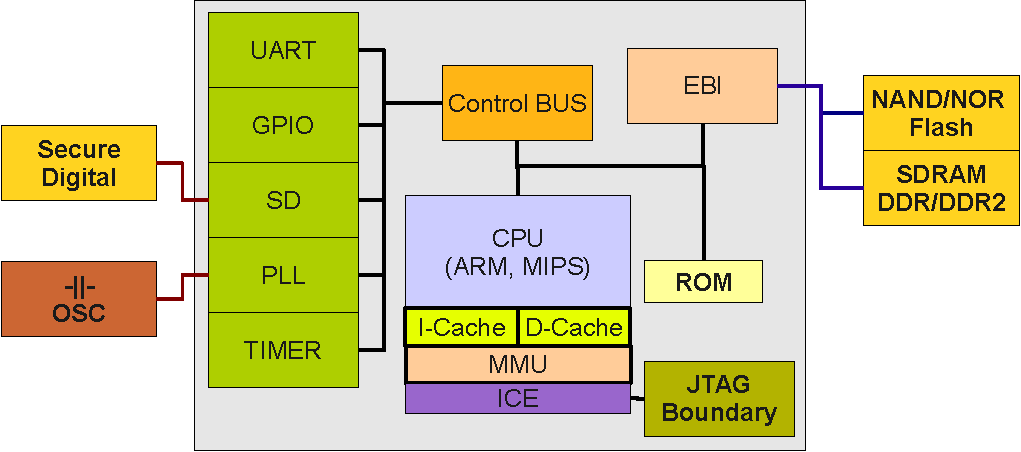
\includegraphics[scale=.45]{../images/soc_no_int_volatil_mmu.pdf} \end{center}
    };



    \onslide<3> \node [ph_explain, right=.5cm of adaptation.east] (exp_adaptation)    
    {
    \begin{center} \textbf{Adaptaci�n: Flujo de dise�o Software} \end{center}
      \begin{center} 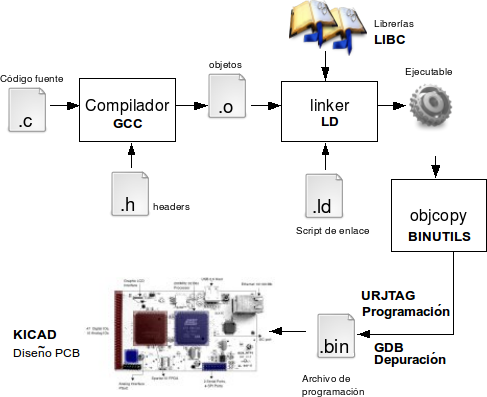
\includegraphics[scale=.6]{../images/SW_design_flow.png} \end{center}
    };



    \onslide<4> \node [ph_explain, right=.5cm of adaptation.east] (exp_adaptation)    
    {
    \begin{center} \textbf{Adaptaci�n: Flujo de Dise�o Hardware} \end{center}
      \begin{center} 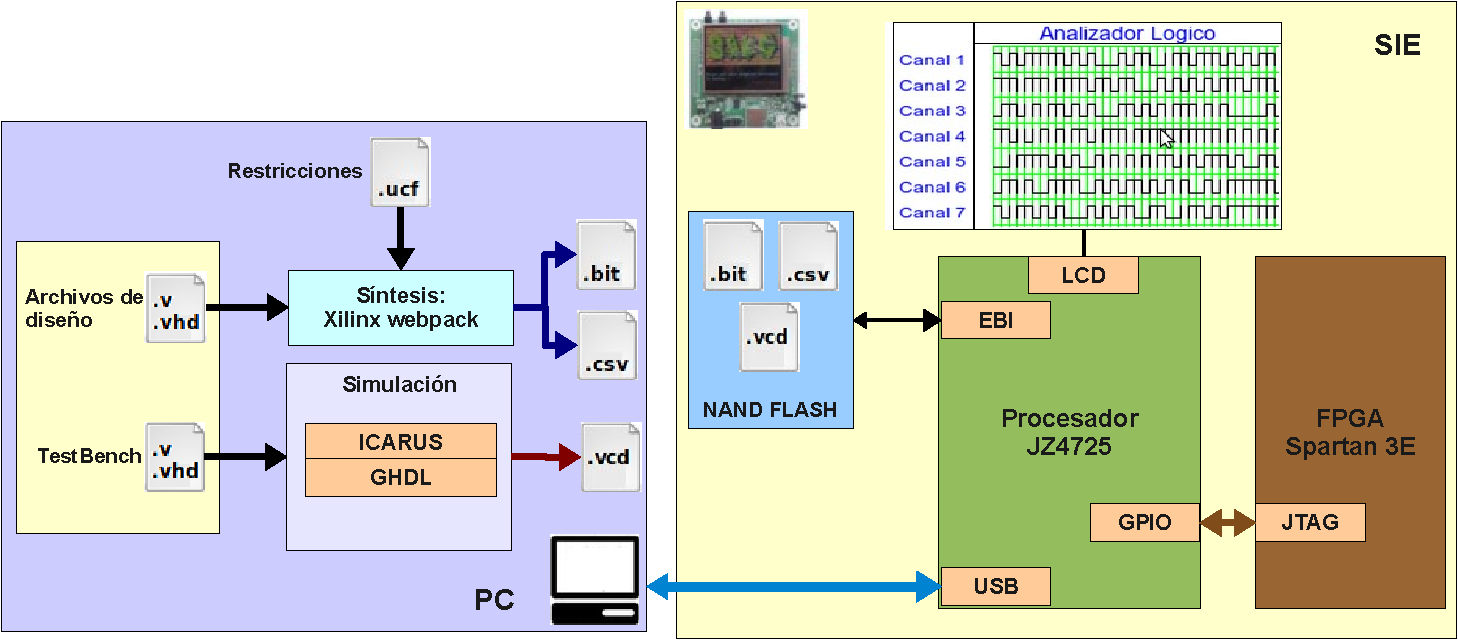
\includegraphics[scale=.35]{../images/HW_design_flow.pdf}   \end{center}
    };




    \onslide<5> \node [ph_explain, right=.5cm of adaptation.east] (exp_adaptation)    
    {

    \begin{center} \textbf{Adaptaci�n: Flujo de Dise�o SoC (softcore))} \end{center}
	\begin{center} 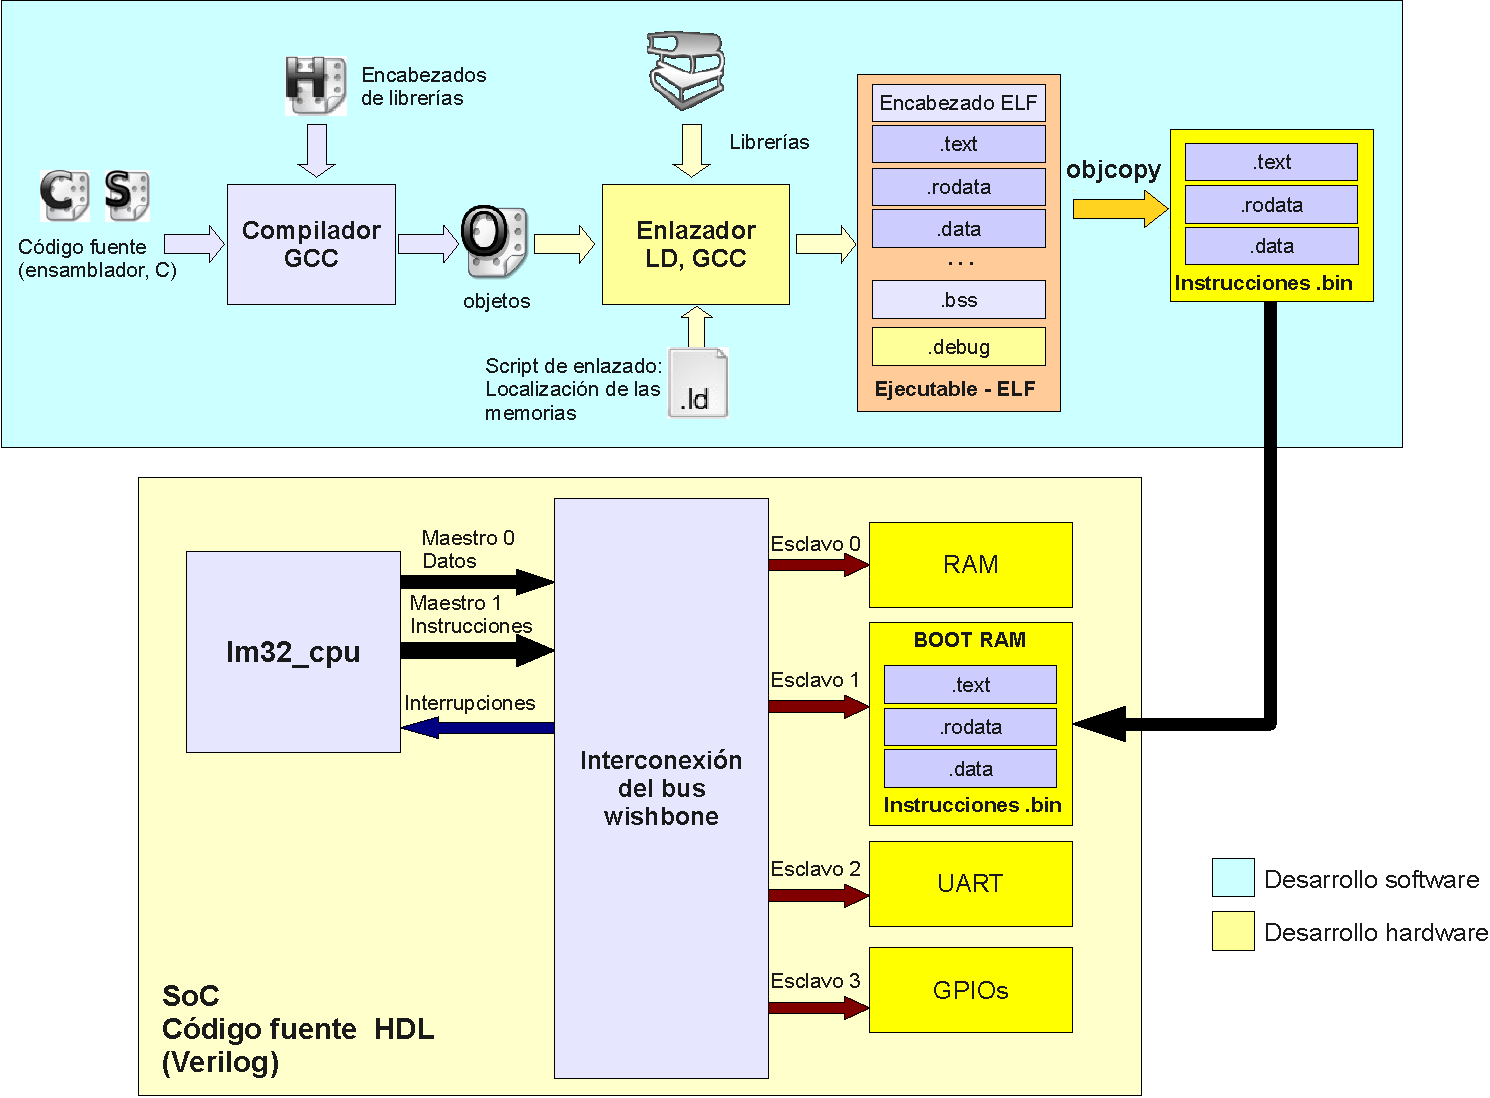
\includegraphics[scale=.35]{../images/soft_SoC_design_flow.pdf}   \end{center}
    };



    \onslide<6> \node [ph_explain, right=.5cm of adaptation.east] (exp_adaptation)    
    {
    \begin{center} \textbf{Adaptaci�n: Conocimientos adquiridos} \end{center}
      \begin{table}[htpb]
        \centering
        \resizebox{!}{1cm}{
          \begin{tabular}{|l|l|l|p{1.6in}|}
            \hline
            \textbf{Plataforma}  & \textbf{Herramientas de desarrollo}  & \textbf{Sistema Operativo y Aplicaciones}
            \\ \hline 
            Game Boy            &ARM GNU toolchian         & eCos, implementaci�n de perif�ricos en FPGAs.
            \\ \hline 
            Zaurus              &ARM GNU toolchian         & Linux 2.4, sistema de archivos, QT.
            \\ \hline 
            iPAQ H3600          &ARM GNU toolchian         & Linux 2.4, Buildroot, QT.
            \\ \hline 
            Chumby              &ARM GNU toolchian         & Linux 2.6, u-boot, OpenEmbedded, QT, flash.
            \\ \hline 
            Ainol V2000         &MIPS - ELF  GNU toolchian & Linux 2.6, openwrt, QT.
            \\ \hline 
            SUNGALE DPF         &MIPS - ELF  GNU toolchian & Linux 2.6, openwrt, QT.
            \\ \hline 
            B\&N NOOK           &ARM  GNU toolchian        & Linux 2.6, Android Dalvik (VM).
            \\ \hline 
          \end{tabular}
         }
      \end{table}
    };


    \onslide<7> \node [ph_explain, right=.5cm of adaptation.east] (exp_adaptation)    
    {
    \begin{center} \textbf{Adaptaci�n: Metodolog�a de dise�o} \end{center}
        \begin{center} 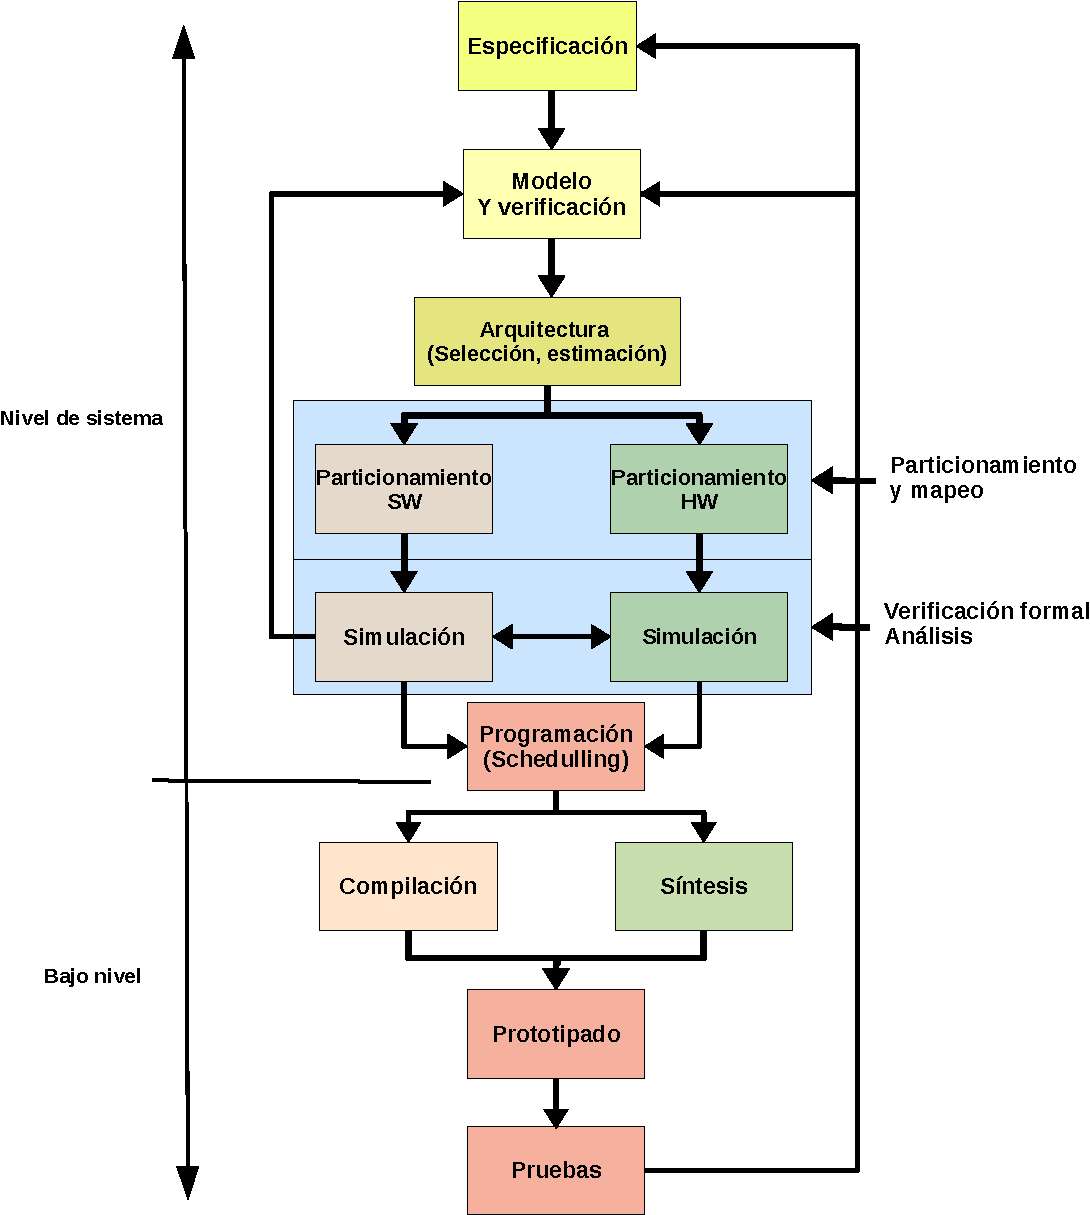
\includegraphics[scale=.41]{../images/embedded_system_design_flow.pdf}   \end{center}
    };
    
\end{tikzpicture}
\end{figure}

\end{frame}


